\documentclass[11pt]{article}
\usepackage[margin=1in]{geometry}
\usepackage{indentfirst}
\usepackage{enumitem}
\usepackage{graphicx}
\usepackage{float}
\usepackage{tikz}
\usepackage{subcaption}
\usepackage{filecontents}
\usepackage{bookmark}
\usepackage{csvsimple}

\begin{document}
\begin{titlepage}
\begin{center}
 {\huge\bfseries Optimizing Culver Academies' Sidewalk Network}

 \vspace{1.5cm}
 {\Large\bfseries Haoxiang Zhang}\\[5pt]

 \vspace{2cm}

 \vfill
 % ----------------------------------------------------------------
{LTC Farmer}\\
{Honors Seminar in Math}\\[5pt]
 \vfill
\today{}
\end{center}
\end{titlepage}
\newpage
\tableofcontents
\section{Abstract}
This study investigates the optimization of the sidewalk network at Culver Academies using agent-based and heuristic algorithms. The goal is to design a pathway network that balances construction costs with traffic demands to improve accessibility for students. Two algorithms are applied: the Slime Mold Algorithm (SMA) and the Union of Rings Algorithm (URA). The SMA generates a network that minimizes total cost but sacrifices clustering and average path length, resulting in fewer direct connections between buildings. The URA, on the other hand, produces a more balanced network with shorter average path lengths and improved accessibility, though at a higher cost. When intersections are added to the SMA model, the network efficiency improves, with reduced average path lengths and better connectivity, though the total cost increases. The study finds that while the SMA is more cost-effective, the URA offers superior path accessibility. These findings offer reflection towards the reasoning behind the existing pathway network and provide a framework for future network design at Culver Academies. 
\section{Introduction}
The Culver Academies is a private boarding school with a long history, established in 1894. Since then, the school has developed and expanded gradually, with new demands and constructions. The road network that has developed in these years is a complex transportation system that is not necessarily developed to fit the needs of students today. \par
Most of the student body at the Culver Academies had probably been shouted at by adults for crossing the grass rather than taking a detour on the sidewalks. This is a result of frustration caused by the designs of the pathways on campus, feeling the irritation of seeing the destination drifting further away as we walked on the sidewalks. The existing pathway system is not necessarily planned for the continued growth of future transportation needs.\par
To make everyday path planning more convenient for students, this paper will explore the various methods to generate and optimize pathway networks in the Culver Academies. Designing an efficient path network has been a challenge due to the interdependent system consisting of discrete nodes. The goal of the designer is to construct a pathway system with minimum cost while satisfying traffic needs for members of the Culver Academies. \par
The problem of designing a network to meet certain constraints while optimizing specific characteristics draws similarities to many real-life applications in communication networks, water systems, and many other problems that could be modeled by the interactions between discrete individual nodes. This wide range of applications encouraged the development of many approaches. In this paper, I will be investigating the approaches of several agent-based and heuristic algorithms and applying them to the setting of Culver Academies. \par
\section{Background Research}
\subsection{Network Planning}
Designing a network is a complicated optimization problem typically formulated as an Integer Linear Programming (ILP) problem with considerations of performance, reliability, and cost. The discrete nature of the problem makes it a challenging problem to solve, often requiring human experts to set certain standards (Zhu et al, 2021). Many of the design processes and algorithms in network planning are developed to other fields of study, primarily in telecommunications.\par
This type of optimization falls under combinatorial optimization, which is finding an optimal subset of the given set of objects. In this case, the problem is to find the best combination of sidewalks among all possible paths between buildings on Culver Academies by deciding which paths to keep or remove. Non-heuristic optimizers such as linear programming or gradient descent struggle with this discrete nature. Exact methods are also difficult due to their computational complexity. For a set of $N$ buildings, the number of possible subsets of paths is $2^N$, making the problem NP-hard (Schrijver, 2003). \par
Network planning is studied most frequently in telecommunications. In this subject, designing a network starts with designing the topologies with regard to cost. This step outputs the physical network and the locations of intermediate nodes. Then, the traffic will be evaluated to formulate the logical links between nodes (Penttinen, 1999). In this study, there is no difference between the logical and physical, but the process of topological design before optimizing based on traffic can be applied to this problem. \par
\subsection{Graph Theory}
A road network is often represented by a graph, with destinations and intersections as vertices, and roads as edges, denoted as $G=\left(V,E\right)$. $V$ denotes the finite collection of vertices $v_1,v_2,\ldots,v_n\ \in V$ and $E$ denotes the finite collection of edges. An edge connecting two vertices $v_1,v_2$ could be directed, represented by the ordered pair $\left(v_1,v_2\right)$, or can be non-directed, where it can be represented by a set $\{v_1.v_2\}$. While a sidewalk seems to be intuitively non-directed as one can walk in both ways, a directed edge is also useful to represent direction of traffic at certain times.\par
	To better model the geographical distance and traffic capacity of the road network, a weighted graph $\left(G,w\right)$ is used where $G$ denotes the graph representing the road network and w maps every element in $E$ to a real number. In other words, it simply assigns one or more numbers to each edge.\par
	The relationship between nodes can be represented by an adjacency matrix. The adjacency matrix $A$ for a graph $G$ is an $n\ \times n$ matrix. For the vertices $v_1,v_2,\ldots,v_n\in V\left(G\right)$, if $\left(v_i,v_j\right)\in E\left(G\right)$, meaning that there exist an edge for $v_i$ and $v_j$, then $A_{ij}\ =\ 1$, else $A_{ij}=0$. For a weighted graph, $A_{ij}$ can be equal to the weight value. (Griffin, 2023).\par
\section{Methodology}
\subsection{Problem Description}
Given the locations of 30 nodes which represents all buildings on campus and the traffic requirements $t_{ij}$ between them, the problem is the determine which of the $n\left(n-1\right)/2$ possible edges to construct, which means choosing from $2^{n\left(n-1\right)/2}$ possible topologies (Corne et al., 2000). The resulting graph representation is an undirected graph where nodes correspond to buildings and edges correspond to sidewalks. \par
To better fit the problem into a graph theory model, several assumptions are made regarding the graph representation of the path network: 
\begin{itemize}
	\item The path network is a 2-dimensional model, ignoring all elevation changes. 
	\item All paths have the same traffic capacity. 
	\item Only buildings enclosed by Academy Road, State Road 10, and East Shore Drive will be included in this model. 
	\item Obstacles and existing roads are ignored.
	\item Each building is represented by one node, regardless of its size or number of entry points. 
\end{itemize} \par
For simplicity, Lake Maxinkuckee is excluded from the study as it does not contain any buildings inside, so its absence does not disrupt the graph structure. Path distances affected by the lake are ignored.\par
By framing the problem within graph theory, this study aims to explore heuristic algorithms to address the challenges of optimizing discrete, interconnected systems. The solutions are implemented using Python and Jupyter Notebook.\\
\subsection{Data Collection}
The data used in this study is obtained from geojson.io by pinpointing geographical locations of buildings on the Culver campus manually. The result is converted by the website into a geojson file which can be processed in Python. The data contains a total of 30 buildings on the Culver campus. For each building, the converted file contains an index, name, longitude, and latitude that corresponds to it. \par
\begin{figure}[H]
\centering
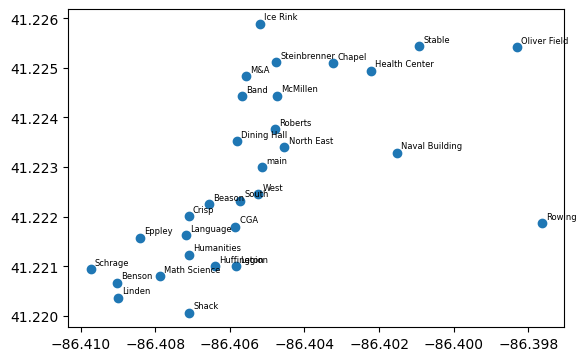
\includegraphics[height=200px]{campuslayout.png}
\caption{The geographical location (longitude and latitude) of the buildings on Culver Academies, labeled with their names.}
\end{figure} 
A set of paths is also collected as edges, they are simplified and collected without considering intersections. This will be used as comparison to generated networks \par
\begin{figure}[H]
\centering
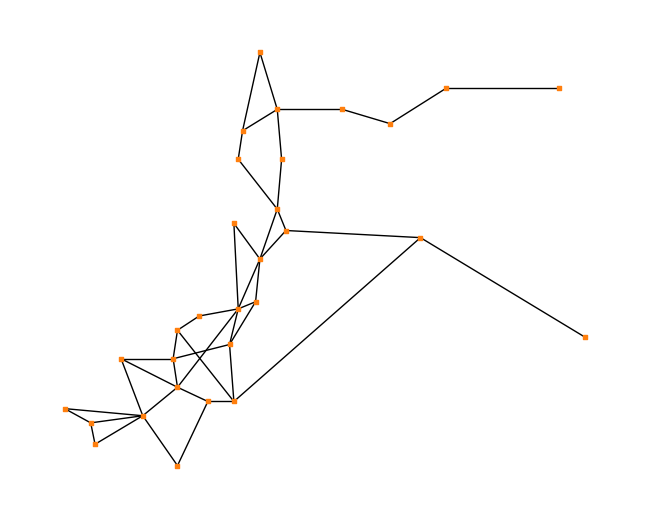
\includegraphics[height=200px]{original.png}
\caption{The graph representation of the pathway network on Culver Academies.}
\end{figure} \par
The geographic dataset is scaled so that each unit length equals to $10^-4$ units of longitude or latitude. The dataset is scaled this way because the SMA works in integer units with the grid simulation, and scaling in this way can make the grid simulation more percise at reflecting actual geographic distance. The Union of Rings Algorithm will also scale the original data in this way to easily compare qualitative results. \par
In the Union of Rings Algorithm, minimum traffic requirement is considered. Therefore, a requirement matrix containing the minimum traffic flows between each pair of nodes is estimated using a set of rules that attempts to reflect actual traffic based on my empirical observations. The rules are as follows:
\begin{enumerate}
\item Traffic requirement will be assigned in values of 1, 3, 5, 10, 15, and 20. 
\item Between each barrack and dorm, the traffic requirement is 10. 
\item Between each barrack and major academic buildings (Humanities, Crisp, Math and Science, and Langauges), the traffic requirement is 10, with the exception of the CGA dorm and Main, which has values of 15. 
\item Traffic requirement for each major academic building to each other is 20.
\item For Legion Memorial, the Library, and Schrage, the traffic requirement is 10 to barracks/dorms and to other academic buildings.
\item The Dining Hall has traffic requirements of 20 to major academic buildings and barracks/dorms. 
\item All sports buildings (except for Oliver field) has a traffic requirement of 10 to barracks/dorms and to the Dining Hall.
\end{enumerate} \par
Other empirical observations from myself is also applied to acquire the resulted requirement matrix. Since the algorithm does not require precise values and focuses more on having uniform numbers, actual traffic data on campus will not be gathered since gathering accurate, real-time, or historical traffic data for each pathway on the Culver Academies campus would require extensive data collection efforts.

\subsection{Slime Mold Algorithm (SMA)}
The slime mold algorithm draws inspiration from \textit{Physarum polycephalum}, a type of slime mold that can form biological networks as a part of their foraging strategy to discover and exploit food sources (Tero et al., 2010). These biological networks have been optimized through many cycles of evolution, making it a reasonable approach to design a transportation network.  \\
\begin{table}[H]
\begin{center}
\begin{tabular}{|l|l|}
\hline
\textbf{Symbol} & \textbf{Description}               \\ \hline
$t$                              & Current Iteration                                   \\ \hline
$P_{max}$                        & Maximum Pheromone Density of a cell                 \\ \hline
$\delta$                         & Decay parameter                                     \\ \hline
$(C_x,C_y)$                      & Current position of a slime cell                    \\ \hline
$(F_x,F_y)$                      & Position of target food                             \\ \hline
$T_1$                            & Moving threshold for primary diffusion              \\ \hline
$T_2$                            & Diffusion thershold for secondary diffusion         \\ \hline
$P_{i,j}(t)$                     & Pheromone level of cell on $(i,j)$ at iteration $t$ \\ \hline
$d$                              & Direction of diffusion                              \\ \hline
$D$                              & Diffusion decay rate                                \\ \hline
$P_{\mathrm{food}}$                       & Pheromone level when a slime cell reaches food      \\ \hline
$\tau_{i,j}\left(t\right)$                       & State of the cell at $(i,j)$      \\ \hline
\end{tabular}
\caption{Notation used in the slime mold algorithm}
\end{center}
\end{table}
The slime mold algorithm can effectively model the pathway network by mimicking how slime mold forms efficient nutrient pathways between food sources. In this study, each building, or node, is represented as a food source that attracts slime cells. The direction-based exploration mechanism simulates the natural preference of shorter, direct paths by penalizing longer or redundant paths with pheromone decay. The reinforcement of the paths optimizes the cost of the pathway system. \par
The slime mold simulation on the Culver building complex will be implemented using Python, using the model described in Zhang, 2022. The simulated slime mold model, an $N\ \times M $ lattice graph $G=\left(L,E\right)$, where L is the set of cells for the $N \times M$ lattice. In the simulation, the dimension of the lattice graph is determined by the maximum horizontal and vertical distance between buildings on Culver Academies.  \par
An individual cell contains its location index $\left(i,j\right)$, its current state, and its pheromone density. Each cell can have one of the following states at a given iteration $t$, represented as $\tau_{i,j}\left(t\right)\in\{0,1,2\}$. \\
\begin{itemize}
\item 0 - Empty: Cells without any food or slime.
\item 1 - Slime: Cells that are considered part of the slime mold.
\item 2 - Food: Cells containing food source, representing the nodes of the pathway network. 
\end{itemize} \par
In the simulation, an initial slime is placed onto one arbitrary food cell to start. It will then start searching for nearby unconnected food sources. Each slime cell, although viewed together as a single organism, is modeled as an individual agent, making its own decisions based on local inputs. Each slime cell will first gather the shortest path to the nearest food source, and will diffuse, by replicating into neighboring cells, following these four features (Zhang, 2022):
\begin{enumerate}
\item Diffusion into another cell decreases that cell’s pheromone density. 
\item The slime will prioritize diffusing to a neighboring cell closest to shortest path to the food source. 
\item The slime will not diffuse if it is too far from a connected food source, or if the target cell’s pheromone level is too low. 
\item The slime’s decision will also be affected by the state of the neighboring cell: food, empty, or slime. 
\end{enumerate} \par
The diffusing mechanism can be categorized into primary and secondary diffusion, where primary diffusion occurs along the shortest path towards the food source, and secondary diffusion occurs when primary diffusion is blocked. 
Before diffusion happens, from all 8 possible directions (positive and negative directions along the horizontal, vertical, or diagonal), one or more direction indices $d$ is selected if the direction points to a food source. These indices are set as the primary direction for a slime cell. \par
Diffusion occurs when the pheromone level in the slime cell exceeds the moving threshold $(P_{C_x,C_y}\left(t\right)> T_1)$, the slime cell attempts to initiate primary diffusion to the neighboring cell denoted by $\left(k,l\right)$. If the cell $\left(k,l\right)$ lies within the lattice grid $G$ and is empty, the diffusion will begin by setting $\left(k,l\right)$ to a slime cell. \par
Secondary diffusion occurs when the slime cell cannot diffuse along the primary direction. Secondary diffusion is random and occurs when the distance if its distance to the nearest food is smaller than the diffusion threshold ($T_2$) (Cai et al, 2020). This process is much slower to reach a food source in order to favor primary diffusion, which uses the shortest distance. \par
 For every iteration during diffusion, an amount of pheromone is lost in a slime cell. The pheromone level of the starting cell is updated by this exponential decay function, where $D$ is the diffusion decay rate and $\delta$ is the decay parameter:
\[ P_{C_x,C_y}\left(t+1\right)=P_{C_x,C_y}\left(t\right)\cdot\left(1-D\ \cdot\delta\right)
\] \par
By diffusing into the neighboring cell $\left(k,l\right)$, the slime mold deposits an amount of pheromone to the new slime cell since an empty cell has no pheromone. The pheromone level is updated as follows to ensure that the level of pheromone does not exceed the maximum level $P_{max}$ (Zhang, 2022): \par
\[ P_{k,l}\left(t+1\right)=min{\left(P_{k,l}\left(t\right)+\frac{P_{C_x,C_y}\left(t\right)}{D},P_{max}\right)} \] 
This same function is used when a slime cell has less pheromone than its neighbor to simulate the transfer of nutrients from a food source. \par
	If any slime cell becomes adjacent to a food cell during an iteration, its pheromone level is instantly set to a fixed value $P_{\mathrm{food}}$. This represents a reward for finding food. This means that if the slime connects 2 food sources, the connection will be maintained with sufficient pheromone, creating a path between two buildings. In the simulation, a trial of high pheromone concentrated cells between 2 food sources will be recognized as a path between 2 buildings.  \par
The processes described above will continue until it reaches the maximum iteration set at the beginning of the simulation. \par
During diffusion, the slime mold system will decay simultaneously based on its distance to a connected food source and pheromone density of the cell it is on. The diffused slimes will deliver nutrients to other food sources and increase pheromone levels in this process. If a slime cell has a pheromone level below a certain point, it will decay into an empty cell. This process ensures that only the most efficient nutrient pathways are kept (Li, et al, 2020). \par
To model this, the activity of the slime cell is directly tied to its pheromone level so that if no exterior pheromone from the food sources is provided, it cannot move to a new location through diffusion and becoming inactive. Therefore, to determine the best path generated by the slime mold algorithm, I would only have to look at if any two food sources is connected by a continuous track of slime cells with high levels of pheromone. \par
The slime mold simulation is visualized step by step. Figure 2 shows the slime mold’s behavior during exploration and the diffusion-decay process to form paths. \par
Since the parameters of the Slime Mold Algorithm does not directly correlate to the qualitative criteria in Section 4.7, I will be performing a parametric study with varying decay values to evaluate its effect on the network generated. 
\begin{figure}[H]
\centering
\hspace*{-1cm}
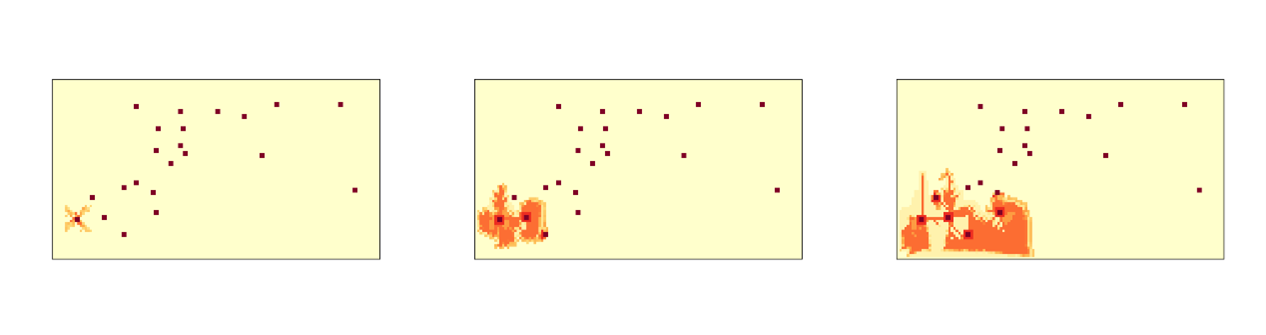
\includegraphics{exampleSMA.png}
\caption{First 50 steps of the SMA on the Culver geographic dataset. Darker orange represents a higher concentration of pheromone.}
\end{figure}
In the simulation, a trial of pheromone concentrated cells between two food sources will be recognized as edges to the network connecting two nodes, resulting in a graph network which can be interpreted as pathway networks on campus.
\par
Since the SMA's parameters do not directly link to the qualitative criteria of graph networks, I will conduct a parametric study with varying decay values in an attempt to generate networks adapted to different balances in constraint. Decay values determine how quickly pheromone levels dissipate, directly influencing the exploration behavior and connectivity of the slime mold. In the context of Culver Academies, adjusting decay values allows the algorithm to simulate different design priorities, such as cost-effectiveness and accessibility. By examining the effects of different decay rates, the study aims to identify an optimal balance between these competing objectives, providing insights into how the algorithm adapts to varying constraints and requirements of the campus environment. \par
\subsection{Union of Rings Algorithm}
Besides the agent-based SMA model, another approach is through heuristic algorithms, such as the Union of Rings Algorithm. This method is described first by Frank and Frisch (1971) and optimized by Blessings (1999) to construct the Minimum Weight Flow-Equivalent Graph (MWFEG). The significance of the MWFEG is that it satisfies the flow requirements under minimum cost, meaning that it is optimal under cost conditions. Another important property of the MWFEG is that it is a biconnected graph, meaning that if any vertex is removed, the graph is still connected (Blessings, 1999). \par
	The algorithm was intended to be applied to telecommunications networks, which, compared to transportation networks such as the one required for this problem, prioritizes reliability and puts less importance on geographical proximity. In this study, the algorithm will be adjusted to prioritize distance constraints over reliability. This adjustment is implemented in Step 1.  \par
The union of rings algorithm follows these procedures to construct the MWFEG outlined by Blessings (1999): \\
\begin{enumerate}
	\item Draw the requirement matrix $R$ that represents the graph $G$ as a complete graph where every vertex is connected, and each edge $\left(i,j\right)$ is labeled with the minimum traffic requirement between nodes $i$ and $j$. In this study, geographical distance is combined with traffic requirement to form a combined matrix $C$ which will be used instead. 
	\item Construct the maximum spanning tree $T$. A spanning tree is a graph that connects all nodes without cycles. For a maximum spanning tree, the total edge weights (from the combined matrix) are maximized, meaning that paths with the highest traffic demands are prioritized.
	\item Convert $T$ into a linear flow equivalent graph $L$. The graph $L$ is flow-equivalent to the maximum spanning tree $T$, meaning that $L$ satisfy the properties that $T$ has in terms of traffic requirements while reducing the cost and complexity of the network.
	\item Factor $L$ into several uniform capacity rings (subgraphs or cycles with equal flow demand). The creation of each ring reduces the traffic of each edge can be reduced by half since each linear flow can now be divided into a 'clockwise' and 'counterclockwise' flow on the ring.
	\item Combine the rings from the previous step with the linear flow graph to create the network topology $N$. The generated topology $N$ will be biconnected, meaning that every node in the network is connected by at least two independent paths, providing robustness to the network. 
	\item Optimize the resulting graph manually to remove insufficient edges or add additional shortcuts. 

\end{enumerate} \par
Step 3 follows these steps to convert the maximum spanning tree $T$ to the flow equivalent graph $L$ (Blessings, 1999):
\begin{enumerate}[label=\alph*.]
	\item Initialize $L$ to be an empty graph and set all nodes in $T$ as unmarked. 
	\item Select an arbitrary node in $T$, mark it, and add it to $L$. This will be the starting node for $L$.
	\item While $T$ contains unmarked nodes: \begin{enumerate}[label=\roman*.]
		\item Identify all edges in $T$ that connect a marked node to an unmarked node.
		\item Select the edge with the maximum weight.
		\item Add the selected edge to $L$. 
	\end{enumerate}
	\item Mark the unmarked node at the other end of the edge and add it to L.
\end{enumerate} \par
$T$ is converted to $L$ in this algorithm because to ensure that redundant edges can only be applied to the most effective places. The linear graph's simple structure minimizes unwanted redundancy that a tree might contain. \par
The adjacency matrix used to create the maximum spanning tree in this study is a weighted sum of the distance matrix $D$ and the requirement matrix $R$, found in Appendeix 10.2 and 10.3. The distance matrix $D$ should award higher weight for shorter distance. Therefore, the value on the $i$th row and $j$th column of $D$ is calculated by the inverse of the Euclidean distance $d\left(i,j\right)$ between the $i$th and $j$th node and multiplied by 100 to reach a similar degree to the requirement values: 
\[ D_{i,j}=\frac{1}{d\left(i,j\right)}\cdot100 \] \par
Given matrices $D$ and $R$, the adjacency matrix that will be used is calculated as follows: \[ C=w_1D+w_2R \] 
Where $w_1,w_2$ are corresponding weights to $D$ and $R$ and $C$ is the resulting combined matrix.  \par
In this study, I will be assuming the requirement matrix which includes the minimum traffic requirements between buildings on campus. The assumption will simply assign traffic requirements by assigning each connection between buildings values 1, 3, 5, 10, 15, and 20, with higher weight meaning more traffic demand. The discrete numbering used to assign traffic requirement is due to the fact that a uniform capacity ring can only be constructed on edges with equal weight. \par
The resulting Minimum Weight Flow-Equivalent Graph represents a pathway system in Culver Academies. Due to the properties of the MWFEG, the resulting pathway network will have balanced cost, robustness, and traffic capacity. \par
Below shows the detailed process of the algorithm when applied to the dataset, labels on the nodes can be corresponded to buildings in Culver Academies in Appendix 10.1:
\begin{figure}[H]
\centering
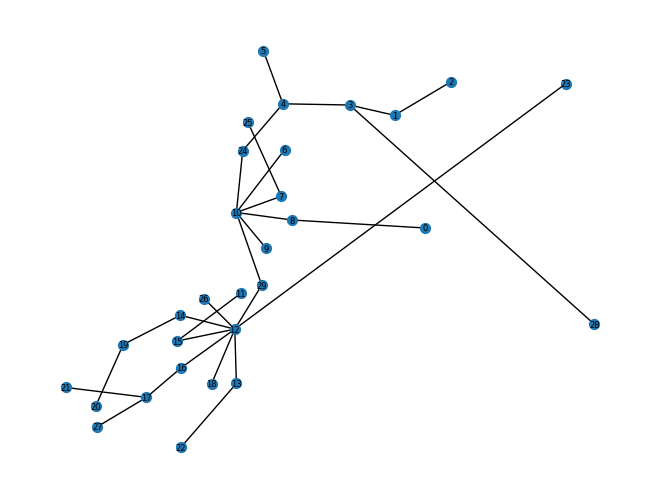
\includegraphics[height=150px]{mst.png}
\caption{The maximum spanning tree from the combined adjacency matrix}
\end{figure}
\par
The maximum spanning tree shown above is generated from a combined adjacency matrix acquired by a weighted sum of the distance and requirement matrix (weights = 1, 0.25 for distance and requirement matrix respectively). The weights are chosen to emphasize on shorter paths, which the original algorithm did not focus on as it is designed for communication networks, and also not completely ignoring traffic requirements. 
\begin{figure}[H]
\centering
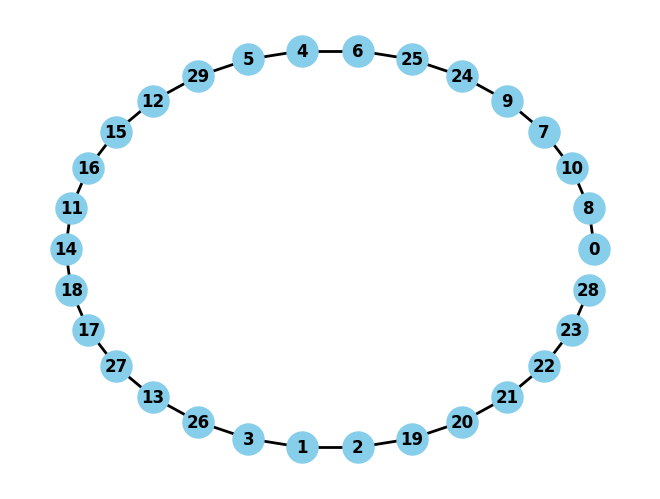
\includegraphics[height=150px]{lfg.png}
\caption{The linear flow graph acquired from the maximum spanning tree}
\end{figure}
\par
The linear graph shown in Figure 5 is linear, meaning that all nodes have degree $\leq$ 1, and maintains all flow properties of the maximum spanning tree, meaning that it is has the maximum possible sum of weights. The above figure shows the linear flow graph labeled with the index of the node. \par
	The uniform capacity rings is extracted from the linear flow graph with weights from the combined matrix, but rounded to discrete values of 1, 5, 10, 15, 20 so that paths with uniform traffic capacities can be easily selected. The rings calculated are shown above in Figures 6. \par
\begin{figure}[H]
    \centering
    \begin{subfigure}{0.32\textwidth}
        \centering
        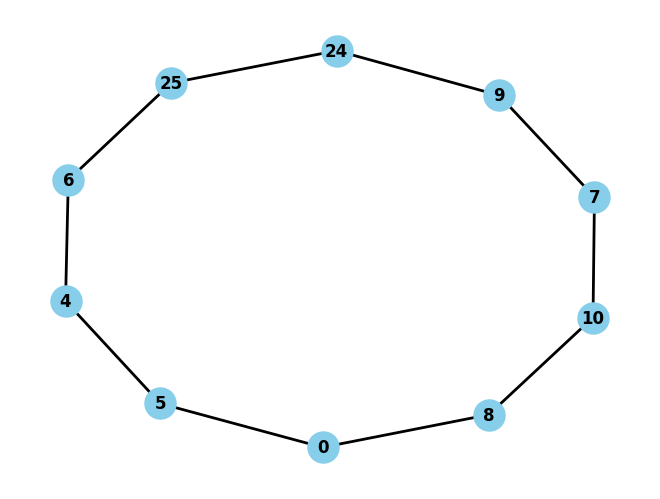
\includegraphics[width=\linewidth]{ring1.png}
        \caption{First Ring}
        \label{fig:ring1}
    \end{subfigure}\hfill
    \begin{subfigure}{0.32\textwidth}
        \centering
        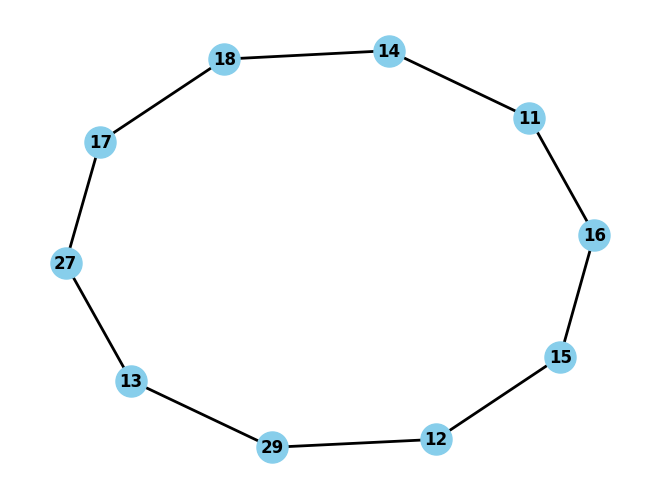
\includegraphics[width=\linewidth]{ring2.png}
        \caption{Second Ring}
        \label{fig:ring2}
    \end{subfigure}\hfill
    \begin{subfigure}{0.32\textwidth}
        \centering
        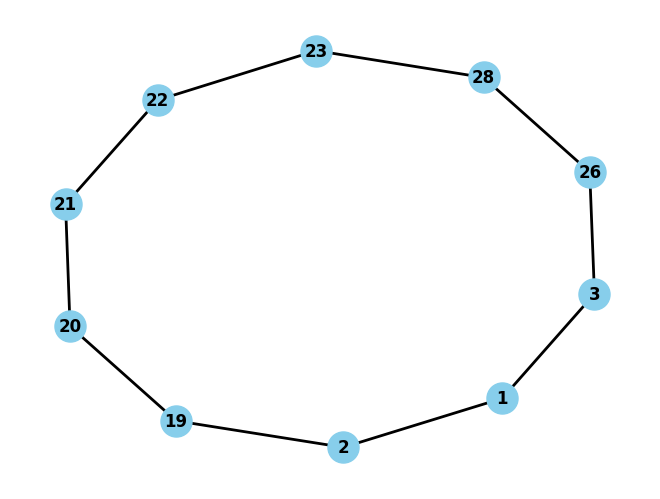
\includegraphics[width=\linewidth]{ring3.png}
        \caption{Third Ring}
        \label{fig:ring3}
    \end{subfigure}
    \caption{Visualization of the three rings generated.}
    \label{fig:rings}
\end{figure}
	These rings are imposed onto the linear flow graph. Creating a combined graph shown in Figure 7.  This is done by inserting any edge that does not exist in the linear graph to the linear flow graph. The uniform capacity rings added to the linear flow graph edges $\left(0,5\right),\ \left(26,\ 28\right),\ \left(29,\ 13\right)$ to the linear flow graph.  (Blessings, 1999). \par
\begin{figure}[H]
\centering
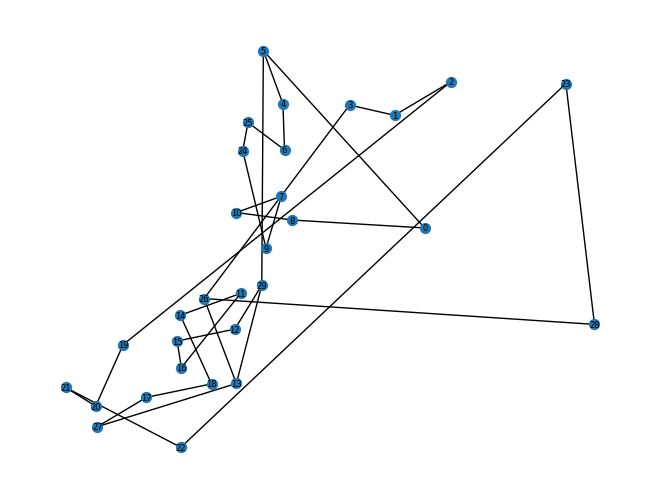
\includegraphics[height=200px]{combined.png}
\caption{The linear flow graph after the addition of rings}
\end{figure}

	Blessings (1999) mentioned to manually optimize the graph by removing insufficient edges. This procedure is implemented in this study through several optimizers, where edges are removed and modified under certain constraints, particularly distance constraints. An edge is removed if its length exceeds 700 units to avoid paths that are unecessarily long. Then if the point to line distance of an edge $\left(u,\ v\right)$ to a node $w$ which it does not connect is less than 45 units, the edge $\left(u,\ v\right)$ replaced by edges $\left(u,\ w\right) and \left(w,\ v\right)$. The processes described above might break the biconnectivity constraint, but since reliability is not one of the key evaluation criteria, it will be placed of a lesser importance. The results of this optimization is shown in steps below.
\begin{figure}[H]
\centering
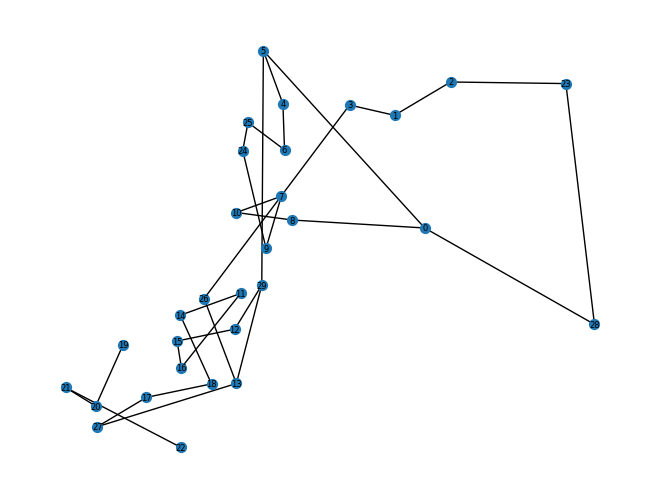
\includegraphics[height=200px]{removelong.png}
\caption{The graph after removing long edges}
\end{figure}
\par The graph above removed long edges such as the path from Oliver Field to the Shack, which was generated from the linear flow graph since these two nodes have little traffic requirements and both far from other nodes. In step 3, these nodes are inefficiently connected together only to maintain a linear flow. 
\begin{figure}[H]
\centering
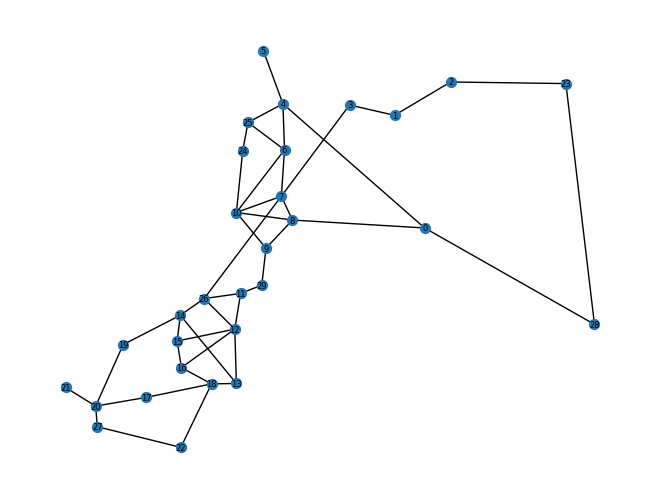
\includegraphics[height=200px]{final.png}
\caption{Final graph after splitting insufficient edges}
\end{figure} 
\par
The graph above created more interconnected path structures as seen in the center of the graph representation. Linear flows from the linear flow graph are converted to more efficient connection patterns by introducing a wider range of degrees compared to a linear pattern, which connects nodes one by one without repetition.
\subsection{Comparison Between the Two Algorithms}
Both the SMA and Union of Rings Algorithm provide a topology of the pathway system for Culver Academies that has a balanced cost and flow. Since the network planning problem has multiple criteria, neither algorithm can guarantee a globally optimal solution. The SMA offers a decentralized, self-optimized approach where the algorithm “learns” the optimal paths over time. Meanwhile, the Union of Rings Algorithm requires a predetermined traffic requirement, but its optimization process is more transparent since it is based on mathematical standards. The Union of Rings Algorithm and the SMA provides a comparison between a globally optimized method and a more locally optimized method (Blessings, 1999). \par
	Since both algorithms are heuristic, they allow for improved flexibility during optimization, making it capable of handling non-linear and discrete constraints in this problem. 
\subsection{Intersections}
Currently, the dataset only includes locations of buildings as nodes. In application, intersections between roads are made to shorten travel distance, distribute traffic and reduce overall cost. Intersections can also be represented by nodes, but its location must be calculated rather than collected. These points that are added to optimize computations are known as Steiner points. \par
	In this study, the intersections in the pathway system are calculated using a Voronoi diagram. The Voronoi diagram partitions a plane containing n points into polygons such that each polygon contains one point and any point on the polygon is closer to the point that it contains than to any other (Weisstein). This makes the edges and vertices of the polygons a reasonable location to place intersection nodes. In this study, the intersection nodes will be placed on vertices of Voronoi polygons as it would have equal distance to at least 3 other nodes. \par
Shown in Figure 10, the Voronoi diagram divides the campus into zones of influence for each building. \\
\begin{figure}[H]
\centering
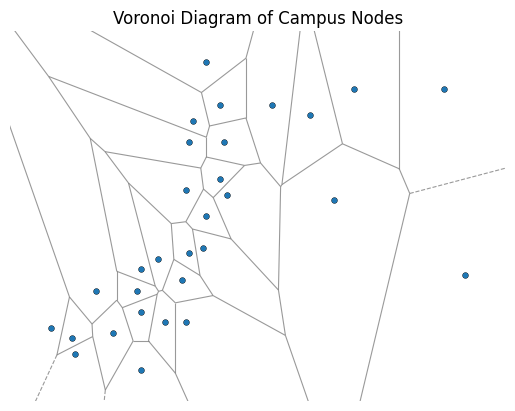
\includegraphics[height=200px]{voronoi.png}
\caption{Voronoi diagram of the graph with buildings on campus}
\end{figure}
\par
To avoid redundancy, the intersection node will only be placed when there is no other intersection node within a radius of 5 units. The intersection nodes will also not be placed when its distance to the nearest building node exceeds 15 units. These parameters are selected from a series of adjustments as they yielded the best result, with no intersections not surrounded by at least 3 buildings and no redundant intersections that occupy similar positions.\\
\begin{figure}[H]
\centering
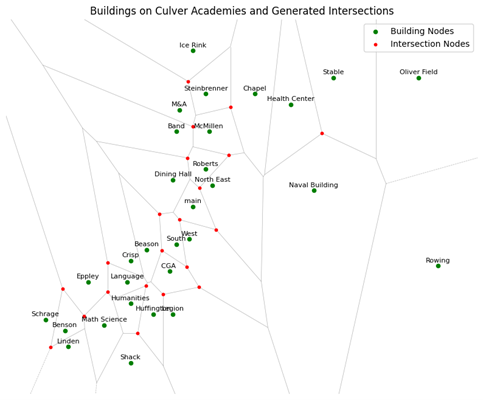
\includegraphics[height=170px, width=300px]{intersections.png}
\caption{Intersections added into the dataset}
\end{figure}
\par
	The resulting graph representation with intersections added is shown above in Figure 11. This model will be used to generate paths in only the SMA algorithm as traffic requirements are undefined for intersections.
\subsection{Evaluation Methods}
Several criteria can be used to evaluate the effectiveness of a transportation network. This study will focus on the quantitative statistics of the graphs, particularly their clustering coefficients, average path length, and total cost of the pathway system. An ideal graph model should satisfy the “small world property”, which includes two criteria to evaluate a graph model: clustering and path length. Models that can produce graphs with higher clustering and shorter path lengths are better (Downey, 2018). In this case, higher clustering means that buildings are connected more directly, while a shorter path length allows people to take less time to reach their destinations. Clustering coefficients and mean path lengths are determined using the open-source Python module NetworkX. \par
	The clustering coefficient is a measure of how interconnected the nodes in the graph are; it measures the likelihood that a node's neighbors are also connected to each other. The clustering coefficient $C_i$ of a node $i$ with $k_i$ neighbors is calculated by:
\[C_i=\frac{2\times\mathrm{number\ of\ edges\ between\ neighbors\ of\ } i}{k_i\times\left(k_i-1\right)}\] 
Where $C_i$ is a value between 0 and 1, with 0 meaning that none of the neighbors of $i$ are interconnected, and 1 meaning that all neighbors of $i$ are interconnected. In this study, I will look at the average clustering coefficient for all nodes in the graph. In a graph with $N$ nodes, the average clustering coefficient $C$ is given by: 
\[C=\frac{1}{N}\sum_{i=1}^{N}C_i\] \par
 	To evaluate the efficiency of the pathway network, the mean shortest path length can be used. It measures the average shortest path in the pathway network between 2 arbitrary buildings. The formula of mean distance L, given the network’s graph model $G=\left(V,E\right)$, is:
\[L=\frac{1}{\left|V\right|\cdot\left(\left|V\right|-1\right)}\sum_{i\neq j} d\left(i,j\right)\] 
Where $\left|V\right|$ is the number of nodes in the graph and $d\left(i,j\right)$ is the shortest path distance between nodes $i$ and $j$. \par
The cost of the network is also evaluated. The cost of constructing a pathway is assumed to be linearly correlated to its Euclidean distance between the connected buildings. Therefore, we can calculate cost using the total distance of edges with the following formula:
\[ Cost = \sum_{i\neq j} d\left(i,j\right) \] \par
	Another way of evaluating a graph is analyzing the probability distribution of the degrees of nodes (how many edges a node is connected to). A PMF (Probability Mass Function) to degree chart will be created to reveal node connectivity patterns. For instance, a scale-free network, where connections are concentrated on a few nodes, follows a power-law distribution. Meanwhile a random network, which is the case for most transportation networks, follows a Poisson distribution (Nykamp).  
\begin{figure}[H]
\centering
\hspace*{-2cm}
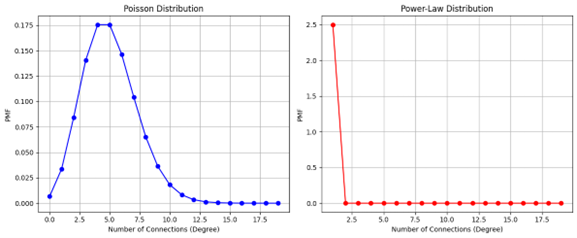
\includegraphics[height=200px]{exdist.png}
\caption{Examples of Poisson distribution and power-law distribution in the context of graphs.  }
\end{figure}
\section{Results}
\subsection{Slime Mold Algorithm}
The slime mold simulation used in this study produces step-by-step simulations. This simulation scaled the dataset to a grid where each unit corresponds to 10-4 degrees in both latitude and longitude on a under decay($\delta$)=0.15. Figure 6.1.1. depicts 4 screenshots of the simulation after 50, 150, 250, and 350 steps, as well as their corresponding graph network. 
\begin{figure}[H]
    \centering
    \begin{subfigure}{0.24\textwidth}
        \centering
        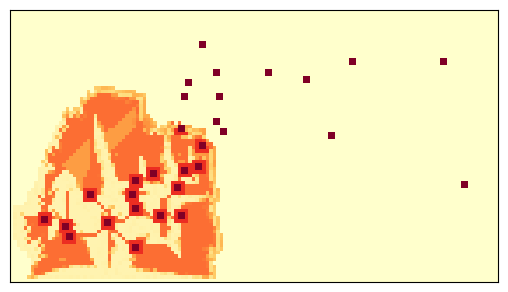
\includegraphics[width=\linewidth]{50steps.png}
	\begin{subfigure}{0.24\textwidth}
	    \centering
	    \hspace*{-1cm}
	    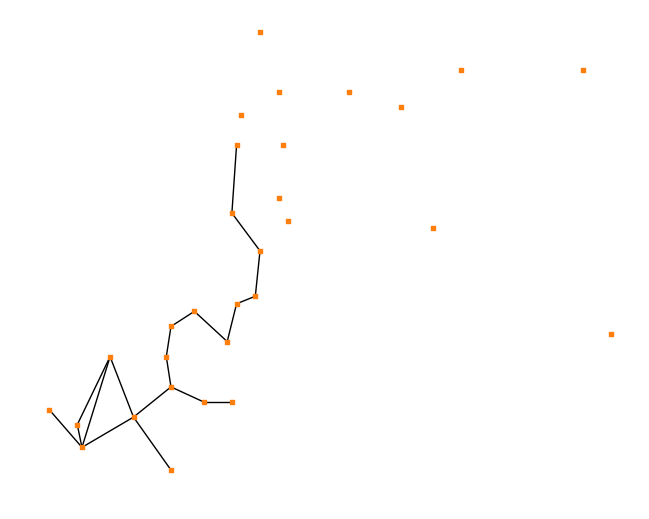
\includegraphics[width=100px]{50graph.png}
	\end{subfigure}
        \caption{50 steps}
    \end{subfigure}\hfill
    \begin{subfigure}{0.24\textwidth}
        \centering
        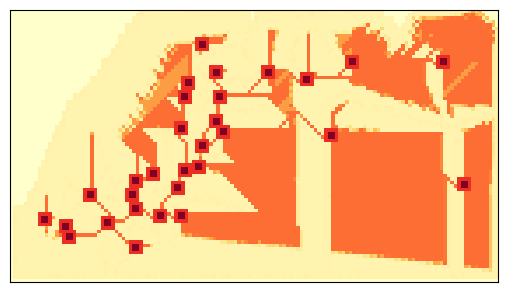
\includegraphics[width=\linewidth]{150steps.png}
	\begin{subfigure}{0.24\textwidth}
	    \centering
	    \hspace*{-1cm}
	    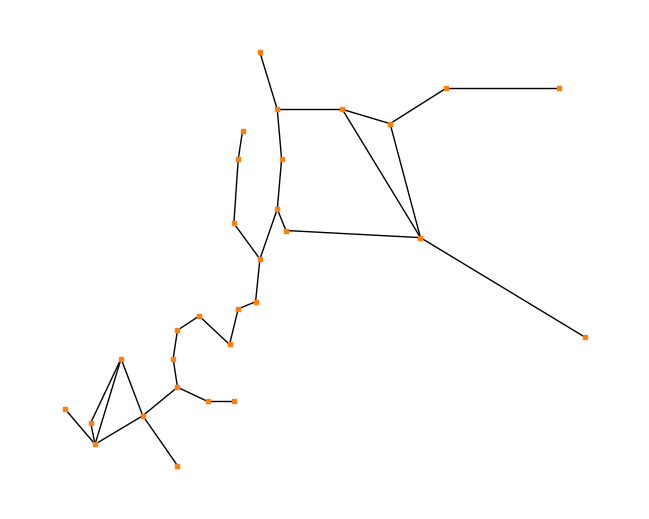
\includegraphics[width=100px]{150graph.png}
	\end{subfigure}
        \caption{150 steps}
    \end{subfigure}\hfill
    \begin{subfigure}{0.24\textwidth}
        \centering
        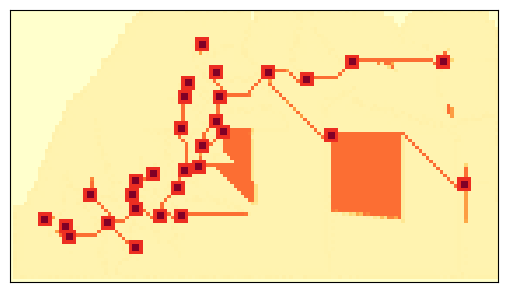
\includegraphics[width=\linewidth]{250steps.png}
	\begin{subfigure}{0.24\textwidth}
	    \centering
	    \hspace*{-1cm}
	    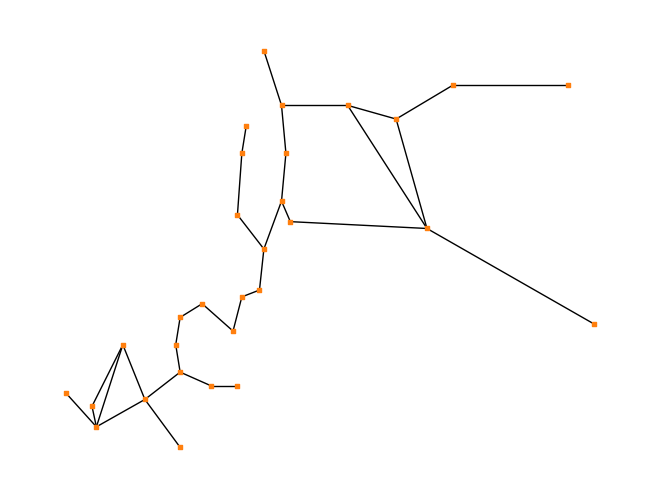
\includegraphics[width=100px]{250graph.png}
	\end{subfigure}
        \caption{250 steps}
    \end{subfigure}
    \begin{subfigure}{0.24\textwidth}
        \centering
        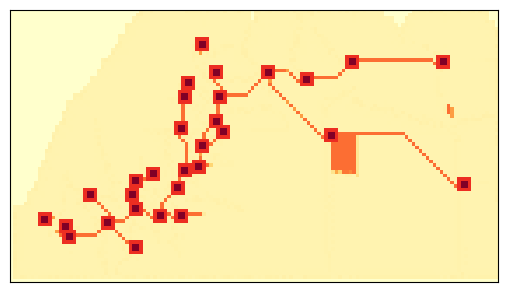
\includegraphics[width=\linewidth]{350steps.png}
	\begin{subfigure}{0.24\textwidth}
	    \centering
	    \hspace*{-1cm}
	    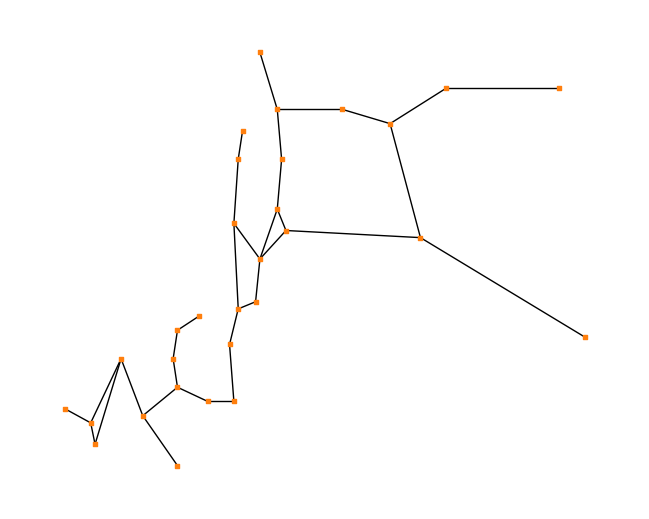
\includegraphics[width=100px]{350graph.png}
	\end{subfigure}
        \caption{350 steps}
    \end{subfigure}
    \caption{Visualization of the slime mold simulation.}
\end{figure}
\begin{table}[H]
\begin{center}
\begin{tabular}{|l|l|l|}
\hline
                         & Original Graph & Slime Mold Graph \\ \hline
Clustering Coefficient   & 0.294047       & 0.130434         \\ \hline
Avg. Path Length         & 4.193103       & 6.744827         \\ \hline
No. of Edges             & 45             & 33               \\ \hline
Total Path Length (Cost) & 525.316170     & 343.959840      \\ \hline
\end{tabular}
\caption{Comparison of evaluation criteria between the original and resulted graph}
\end{center}
\end{table}
\par
Table 2 shows the comparison between the graph connected by the slime mold and the original graph from Culver Academies’ existing pathway system. We can observe that the generated graph resulted in a much different pathway network compared to the original system. Overall, the original system is a better model with regards to the “small world properties” but had significantly more cost. \par
This outcome reflects the trade-offs inherent in the SMA. By focusing on cost minimization, the algorithm prioritized efficiency over accessibility, resulting in fewer connections and longer average travel distances. In the context of Culver Academies, this suggests that while the SMA provides a viable low-cost alternative, it may fail to meet the social and logistical needs of a vibrant campus, where quick and direct access between buildings is often essential. Consequently, while the SMA serves as a useful baseline, further refinements might be necessary to achieve a more balanced pathway network. In this study, I will investigate the effects of different decay values on the cost-efficiency balance of the SMA.  \par
\begin{figure}[H]
\centering
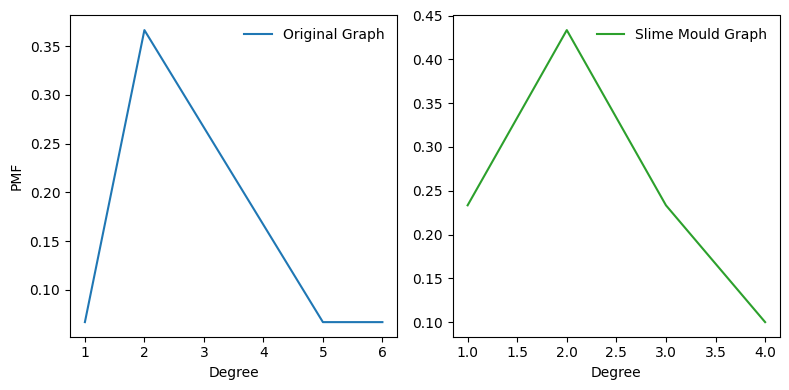
\includegraphics[width=\linewidth]{pmfslime.png}
\caption{PMF graph of the slime in scale. Y axis is node density.}
\end{figure}
Figure 13 shows that the original system contained nodes with higher degrees, which indicates that the original system traded cost for better access and robustness. Both the original and generated graph follow Poisson distribution, indicating that both graphs are random graphs. \par
To test if SMA could satisfy different cost-efficiency constraints, a parametric study is conducted on different decay values. The values tested are 0.075, 0.1, 0.15, 0.2, and 0.25. \\
\begin{table}[H]
\begin{center}
\begin{tabular}{|l|l|l|l|}
\hline
\textbf{Decay} & \textbf{Clustering Coefficient} & \textbf{Path Length} & \textbf{Edges} \\ \hline
0.075          & 0.106667                        & 7.022989             & 32             \\ \hline
0.100          & 0.173333                        & 6.898851             & 33             \\ \hline
0.150          & 0.073333                        & 6.347126             & 33             \\ \hline
0.200          & 0.108696                        & 6.310345             & 33             \\ \hline
0.250          & 0.036232                        & 6.425287             & 33             \\ \hline
\end{tabular}
\caption{Statistics of the parametric study}
\end{center} 
\end{table} 
\newpage
Table 3 shows a comparison of the three decay values under the evaluation criteria. Based on the table, no linear trend can be concluded about decay value and network efficiency (clustering coefficient and mean path length). Little improvement is made from these intervals of decay values. \par
	The number of steps used are collected during network generation for each decay value, shown in Figures 6.1.3 to 6.1.5. These figures suggest that hat as decay values increase, the number of steps required to connect all food sources decreases, which means higher decay values require less iterations than lower values until it reaches a threshold where it is impossible for the slime to reach all food source when pheromone is decaying too rapidly. 
\begin{figure}[H]
    \centering
    \begin{subfigure}{0.32\textwidth}
        \centering
        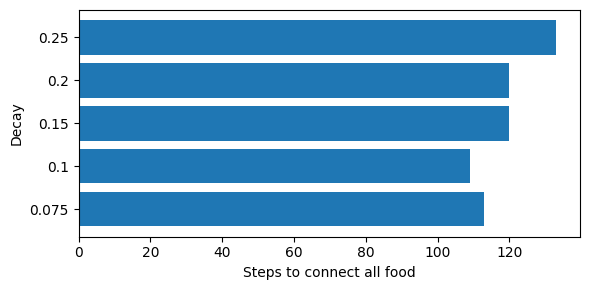
\includegraphics[width=\linewidth]{nostep.png}
        \caption{Number of steps for connecting all foods}
    \end{subfigure}\hfill
    \begin{subfigure}{0.32\textwidth}
        \centering
        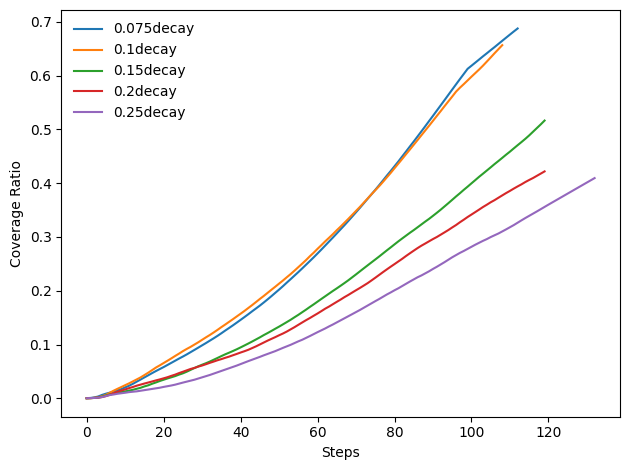
\includegraphics[width=\linewidth]{coverage.png}
        \caption{Slime mould coverage ratio}
    \end{subfigure}\hfill
    \begin{subfigure}{0.32\textwidth}
        \centering
        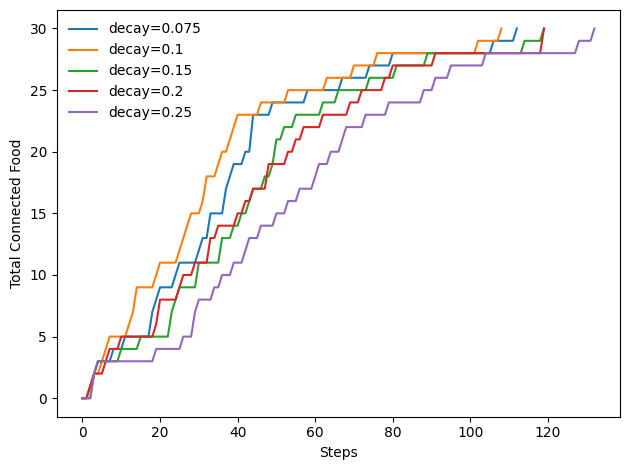
\includegraphics[width=\linewidth]{connectedf.png}
        \caption{Total number of connected food}
    \end{subfigure}
    \caption{Statistics during network generation for the parametric study}
\end{figure}
\subsection{Union of Rings Algorithm}
The Union of Rings Algorithm is applied to the geographic dataset scaled identically with that in the SMA. The generated graph is shown in Figure 16. 
\begin{figure}[H]
\centering
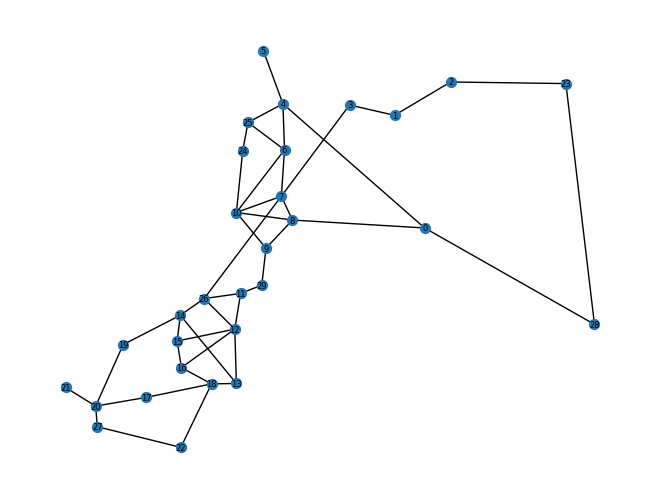
\includegraphics[width=\linewidth]{final.png}
\caption{Output graph from the Union of Rings Algorithm}
\end{figure}
\par
The statistics of the network produced is found in Table 4. 
\begin{table}[H]
\centering
\begin{tabular}{|l|l|l|}
\hline
                           & Original Graph & Graph produced by Union of Rings \\ \hline
Clustering Coefficient     & 0.294047       & 0.112222                         \\ \hline
Avg. Path Length           & 4.193103       & 3.910344                         \\ \hline
No. of edges               & 45             & 44                               \\ \hline
Total Path Distance (Cost) & 525.316170     & 637.945713                       \\ \hline
\end{tabular}
\caption{Statistics of Union of Rings graph}
\end{table}
\par
The statistic of the resulted graph indicates that it had improvements in both total and average path length, creating a sidewalk network with faster access between buildings and lower cost. 
\begin{figure}[H]
\centering
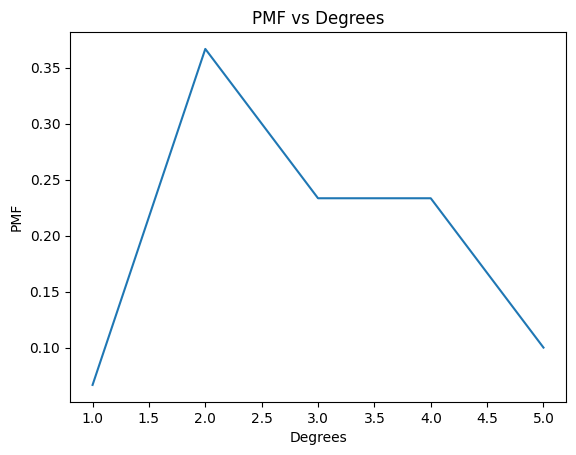
\includegraphics[width=250px]{pmfuor.png}
\caption{PMF graph from the Union of Rings graph}
\end{figure}
\par Based on the PMF shown in figure 17, the Union of Rings graph displayed a wider range of degrees compared to the slime mold graph. This is due to the consideration of traffic requirements set in the Union of Rings Algorithm, creating highly connected hubs such as CGA dorms (node 12) and the dining hall (node 10)
\subsection{Results with Intersections Added}
\begin{figure}[H]
    \centering
    \begin{subfigure}{0.24\textwidth}
        \centering
        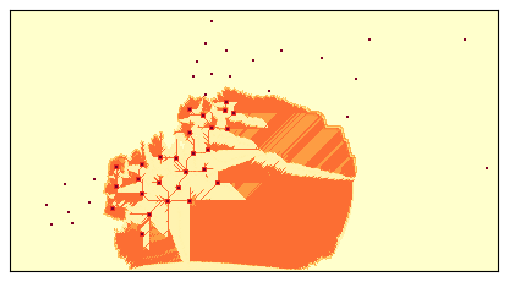
\includegraphics[width=\linewidth]{150.png}
	\begin{subfigure}{0.24\textwidth}
	    \centering
	    \hspace*{-1cm}
	    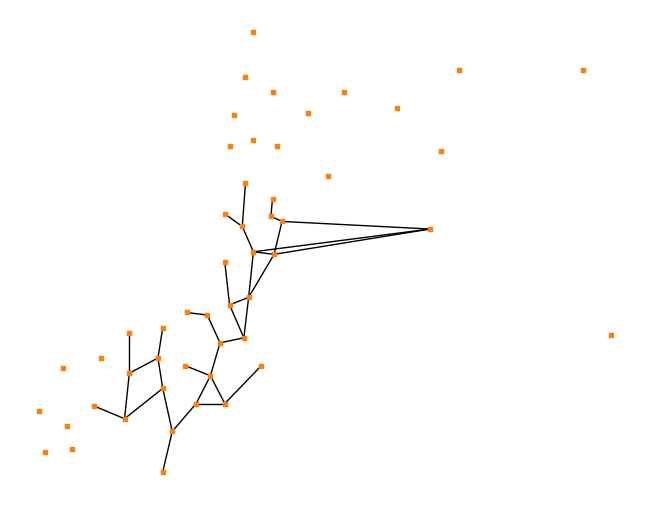
\includegraphics[width=100px]{150g.png}
	\end{subfigure}
        \caption{150 steps}
    \end{subfigure}\hfill
    \begin{subfigure}{0.24\textwidth}
        \centering
        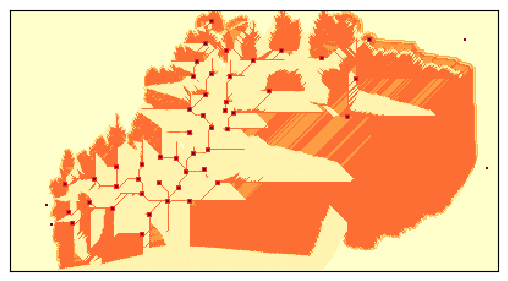
\includegraphics[width=\linewidth]{250.png}
	\begin{subfigure}{0.24\textwidth}
	    \centering
	    \hspace*{-1cm}
	    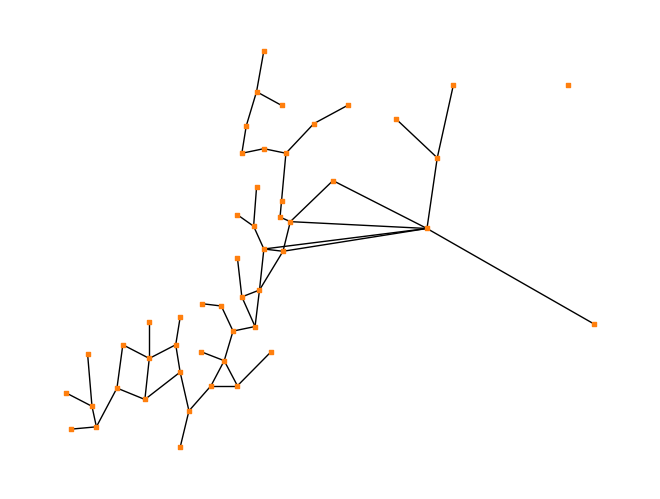
\includegraphics[width=100px]{250g.png}
	\end{subfigure}
        \caption{250 steps}
    \end{subfigure}\hfill
    \begin{subfigure}{0.24\textwidth}
        \centering
        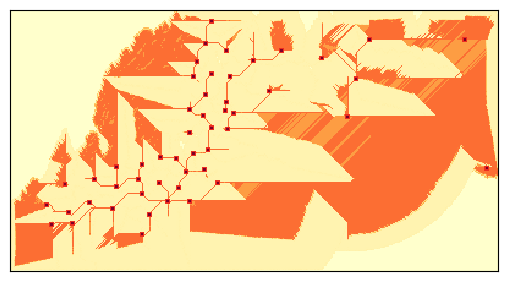
\includegraphics[width=\linewidth]{350.png}
	\begin{subfigure}{0.24\textwidth}
	    \centering
	    \hspace*{-1cm}
	    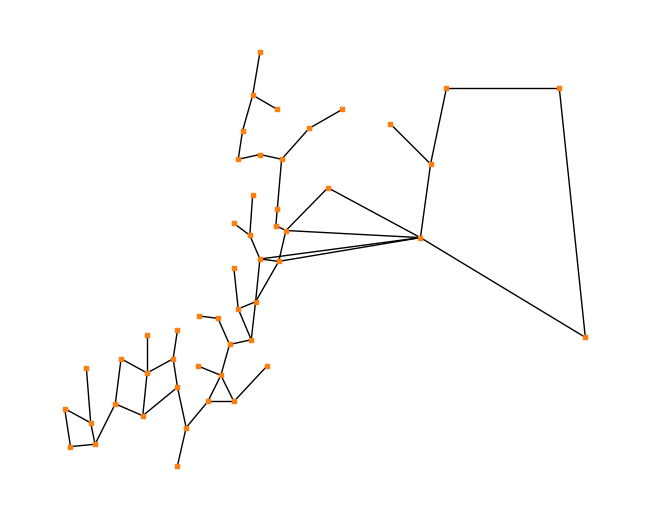
\includegraphics[width=100px]{350g.png}
	\end{subfigure}
        \caption{350 steps}
    \end{subfigure}
    \begin{subfigure}{0.24\textwidth}
        \centering
        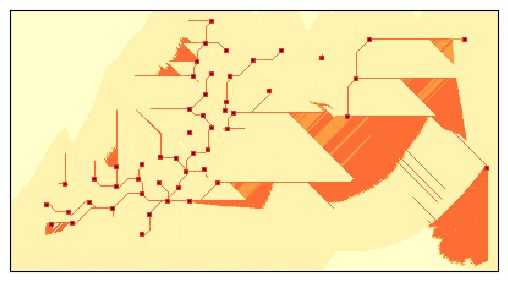
\includegraphics[width=\linewidth]{550.png}
	\begin{subfigure}{0.24\textwidth}
	    \centering
	    \hspace*{-1cm}
	    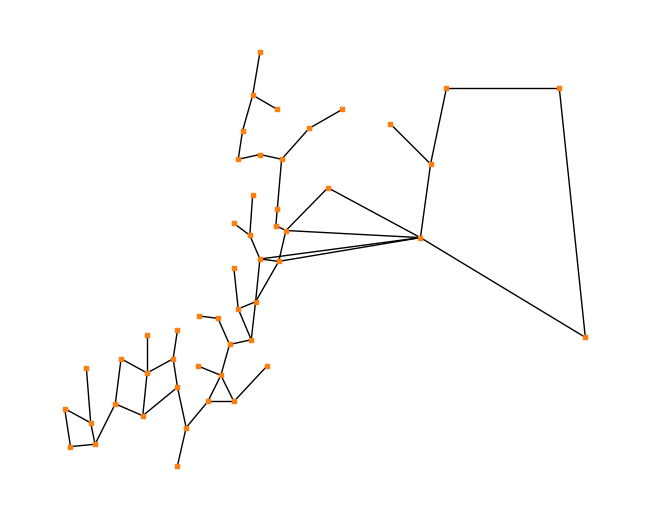
\includegraphics[width=100px]{550g.png}
	\end{subfigure}
        \caption{550 steps}
    \end{subfigure}
    \caption{Visualization the slime mold simulation with intersections added.}
\end{figure}
SMA with intersection is implemented by inputting the graph with intersections to the algorithm. The resulting graph is shown in Figure 18 and statistics are shown in Table 5. 
\begin{figure}[H]
\centering
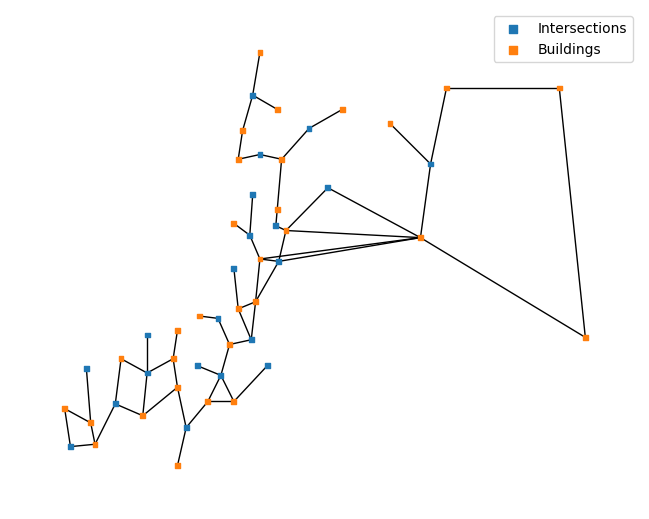
\includegraphics[width=300px]{smainter.png}
\caption{Slime mold graph with intersections}
\end{figure}
\begin{table}[H]
\centering
\begin{tabular}{|l|l|l|}
\hline
                           & Original Graph & Slime mold graph with intersections \\ \hline
Clustering Coefficient     & 0.294047       & 0.113513                            \\ \hline
Avg. Path Length           & 4.193103       & 3.885490                            \\ \hline
No. of edges               & 45             & 60                                  \\ \hline
Total Path Distance (Cost) & 525.316170     & 558.407905                          \\ \hline
\end{tabular}
\caption{Statistics of slime mold graph with intersections}
\end{table}
\par With intersections now added to the input, the slime mold algorithm produced a significantly better graph with better access between buildings. Now two or more paths can share a transportation hub from an intersection and access multiple nodes at once without creating too much connections. From Table 5., we can observe that the slime graph with intersections did allow more connected networks, possibly by reducing the distance between nodes. However, the generated network had 15 more edges, and despite the shorter distances between nodes, this still led to a slight increase in cost. 
\begin{figure}[H]
\centering
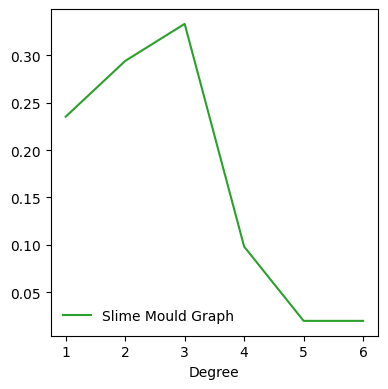
\includegraphics[width=300px]{pmfinter.png}
\caption{PMF graph for slime mold graph with intersections, y-axis is node density}
\end{figure}
\par From Figure 20, there is an increase in degree variety after intersections are placed. Several high connectivity hubs are created. Due to increased degree range, an increase in redundancy can be observed in Figure 19. 
\section{Conclusion}
The sidewalk network constructed using SMA and Union of Rings Algorithm both have comparable, sometimes lower, cost, clustering, and accessibility compared to the original graph, indicating the the two algorithms are capable of generating reasonable and realistic sidewalk networks. However, for the network generated by SMA, the clustering coefficient and mean path length are less than those of the original sidewalk network. Altering decay values does not affect the performance of the network much. In contrast, the Union of Rings Algorithm created a better performing network with an increase in cost compared to the original network and the SMA network. \par
Adding intersections to the SMA increased network efficiency. The intersections increased cost and lowered average path length, shifting to a cost-efficiency balance similar to the original network. However, clustering coeffcient remained similar to the SMA graph without intersections. Intersections proved to shorten path distances by providing a shortcut shared by two or more paths. Placing intersections increased redundancy of paths compared to the SMA graph without intersections by shortening average node-to-node distance. This favored construction of short, low-cost paths that increases connectivity between buildings. 
\section{Future Works}
This study, focused on planning sidewalks in Culver Academies, had provided insights towards network planning. Since traffic is largely ignored in this paper, further studies can investigate the dynamic traffic flows in Culver Academies throughout the day in peak and off-peak hours, such as lunch time or class commutes. Another way to incorporate traffic is to build intersections using a weighted Voronoi diagram, where buildings can be prioritized based on traffic requirements.  \par
The study focused solely on heuristic algorithms. Future studies could explore non-heuristic algorithms particularly those used in objective optimization, where target functions modeling cost and accessibility can be used to determine a global best solution. However, it might be challenging to incorporate the optimizers into a discrete setting. \par
Other methods of creating Steiner points can also be explored. The Voronoi diagram is one of many conventional methods to create intersection points in graph problems. Other methods, such as Delaunay triangulation, focus on different aspects of the graph than the Voronoi diagram, which might produce drastically different results. \par
\section{Lessons Learned}
This study is significantly more difficult than I expected when I started it. The most comprehensive takeaway from this study is the fundamentals of graph theory which I have no exposure to before this study. I also investigated on compuational algorithms during this study, and learned the implications of complexities and how to implement them effectively using Python, specifically with Jupyter Notebook.  I felt that graph theory is a versatile mathematic model that can be applied to a variety of subjects, from transportation networks to social connections. \par
Though not my first time using Python, I furthered my understanding in it by learning to use it in a more interactive setting with Jupyter Notebook. Using Python in this study also deepened my understanding with algorithmic design, as I had to plan out and implement the algorithms in long-term and with an applicative setting. \par
While doing this study, I also learned about my personal approach of working with research papers. I realized that I should conduct more comprehensive research before implementing ideas. In this study, I had to adjust the algorithms several times to produce results clearly because I was not familiar enough with certain aspects of the algorithms used. 
\newpage
\section{References}
Blessing, Jeffery. \emph{Efficient network design using heuristic and
adaptive methods}. 1999. U Wisconsin-Milwaukee, PhD dissertation.
\emph{ProQuest Dissertations and Theses}, \\
www.proquest.com/openview/c5c10c80072655f45d5b720c24c40a50/1. Accessed
19 Nov. 2024.

Cai, Zhengying, et al. "A Node Selecting Approach for Traffic Network
Based on Artificial Slime Mold." \emph{IEEE Access}, vol. 8, 2020, pp.
8436-48, https://doi.org/10.1109/access.2020.2964002.

Corne, David, et al. \emph{Telecommunications Optimization : Heuristics
and Adaptive Techniques}. Wiley, 2000.

Downey, Allen. \emph{Think Complexity}. 2nd ed.,
O\textquotesingle Reilly, 2018.

Griffin, Christopher. \emph{Applied Graph Theory : an Introduction with
Graph Optimization and Algebraic Graph Theory}. World Scientific, 2023.

Lee, Jason. \emph{NETWORK OPTIMIZATION USING LINEAR PROGRAMMING AND
REGRESSION}. 2016. U Oregon, Bachelor\textquotesingle s thesis.
\emph{University of Oregon},
scholarsbank.uoregon.edu/server/api/core/bitstreams/cff1b048-02b6-442a-9eae-3c2a7b170ead/content.
Accessed 1 Oct. 2024.

Li, Shimin, et al. "Slime Mould Algorithm: A New Method for Stochastic
Optimization." \emph{Future Generation Computer Systems}, vol. 111, Oct.
2020, pp. 300-23. \emph{ScienceDirect},
https://doi.org/10.1016/j.future.2020.03.055. Accessed 15 Oct. 2024.

NetworkX Developers. \emph{NetworkX: Network Analysis in Python}.
NetworkX,\\
https://networkx.org/documentation/stable/reference/index.html. Accessed
20 Nov. 2024.

Nykamp, Duane Q. "The degree distribution of a network." \emph{Math
Insight}, mathinsight.org/degree\_distribution. Accessed 20 Nov. 2024.

Penttinen, Aleksi. Lecture. \emph{Helsinki University of Technology},\\
1999, www.netlab.tkk.fi/opetus/s38145/s99/lectures/lect10.pdf. Accessed
6 Oct. 2024.

Tero, Atsushi, et al. "Rules for Biologically Inspired Adaptive Network
Design." \emph{Science}, vol. 327, no. 5964, 2010, pp. 439--42.
\emph{JSTOR}, http://www.jstor.org/stable/40508592. Accessed 15 Nov.
2024.

Weisstein, Eric W. "Voronoi Diagram." \emph{Wolfram Mathworld},
mathworld.wolfram.com/VoronoiDiagram.html. Accessed 17 Nov. 2024.

Zhang, Wenxiao. "CITS4403 Project Report." U of Western Australia, 17
Oct. 2022. \emph{Github},\\
github.com/MoeBuTa/SlimeMould/blob/master/report/report.pdf. Accessed 19 Nov. 2024.

Zhu, Hang, et al. "Network planning with deep reinforcement learning."
\emph{SIGCOMM \textquotesingle21: Proceedings of the 2021 ACM SIGCOMM
2021 Conference}. \emph{ACM Digital Library},
dl.acm.org/doi/10.1145/3452296.3472902. Accessed 6 Oct. 2024.
\newpage
\section{Appendix}
\subsection{Geographic data used in this study}
\begin{table}[H]
\begin{tabular}{|l|l|l|l|}
\hline
index & name           & longitude         & latitude           \\ \hline
0     & Naval Building & 86.40152102911392 & 41.22329034209335  \\ \hline
1     & Health Center  & 86.4022087209599  & 41.22494337522588  \\ \hline
2     & Stable         & 86.40092466867043 & 41.22543548638561  \\ \hline
3     & Chapel         & 86.40323923426236 & 41.225097160360974 \\ \hline
4     & Steinbrenner   & 86.404760468185   & 41.2251156145534   \\ \hline
5     & Ice Rink       & 86.4052006713107  & 41.22589094181927  \\ \hline
6     & McMillen       & 86.40472630804437 & 41.22443921335798  \\ \hline
7     & Roberts        & 86.40478929568881 & 41.22375707874542  \\ \hline
8     & North East     & 86.40453575670179 & 41.223406440924435 \\ \hline
9     & main           & 86.40514269959249 & 41.222993289742135 \\ \hline
10    & Dining Hall    & 86.40582000039917 & 41.22351758367486  \\ \hline
11    & South          & 86.40572156572841 & 41.22232557559556  \\ \hline
12    & CGA            & 86.4058522411408  & 41.22179915379331  \\ \hline
13    & Legion         & 86.40582362655806 & 41.22100530263856  \\ \hline
14    & Crisp          & 86.40710327727534 & 41.22200483416856  \\ \hline
15    & Language       & 86.4071721815452  & 41.221627235163936 \\ \hline
16    & Humanities     & 86.40708359034139 & 41.221234826044366 \\ \hline
17    & Math Science   & 86.40787106770593 & 41.22079799048194  \\ \hline
18    & Huffington     & 86.40639371316998 & 41.2209965122064   \\ \hline
19    & Eppley         & 86.40840178044996 & 41.2215740212541   \\ \hline
20    & Benson         & 86.4090317623419  & 41.22067073562198  \\ \hline
21    & Schrage        & 86.40973064850316 & 41.2209446842225   \\ \hline
22    & Shack          & 86.40709614504999 & 41.22006184559325  \\ \hline
23    & Oliver Field   & 86.3982960667223  & 41.2254099205762   \\ \hline
24    & Band           & 86.40567266803053 & 41.22442373638032  \\ \hline
25    & M\&A           & 86.40555556302346 & 41.22483822289942  \\ \hline
26    & Beason         & 86.40656291338564 & 41.222250039341986 \\ \hline
27    & Linden         & 86.4089958639104  & 41.220368181941495 \\ \hline
28    & Rowing         & 86.39764666670176 & 41.22187152497838  \\ \hline
29    & West           & 86.40524025774005 & 41.22245135491352  \\ \hline
\end{tabular}
\end{table} 
\newpage
\subsection{Processed distance matrix}
\newpage
\subsection{Requirement matrix}
\begin{table}[ht]
\centering
\csvautotabular{"req.csv"} 
\caption{Your Table Caption Here}
\end{table}


\end{document}